%Part of/Parte di https://github.com/f-dinucci/appuntiMeccanicaFluidi/
%License/Licenza Creative Commons Attribution-ShareAlike 4.0 International (CC BY-SA 4.0) - attribution/attribuzione Francesco Di Nucci
%See also/Vedere anche https://creativecommons.org/licenses/by-sa/4.0/ and/e https://creativecommons.org/licenses/by-sa/4.0/legalcode
%
\section{Equazioni di Navier-Stokes} 

\subsection{Quasi equilibrio locale}
Finora è stata fatta l'ipotesi di equilibrio termodinamico locale, che permette di considerare i flussi come funzioni puntuali delle proprietà del fluido nel punto nel quale li si sta calcolando.
In alcuni casi ciò non è possibile e si introduce quindi l'ipotesi di quasi-equilibrio locale: i flussi vengono considerati non più funzioni delle proprietà in un punto, ma delle proprietà \textit{in un piccolo intorno del punto considerato}.

È un'approssimazione ``più precisa'' che considera i flussi funzioni delle proprietà in un punto e dei loro gradienti:
%
	\begin{equation*}
		\uline{J} = \uline{J}_{equilibrio}(\rho, \uline{v}, e) + a \grad{\rho} + b \grad{\uline{v}} + c \grad{e}
	\end{equation*}
%
Se i gradienti sono nulli si torna al caso precedente di equilibrio locale.
Più cresce la dimensione delle molecole, meno la descrizione del fluido come continuo è appropriata, si introdurranno quindi dei numeri adimensionali per distinguere tra i vari casi: cambiano infatti anche le equazioni per descrivere il fluido, passando da quelle di Eulero a quelle di Navier-Stokes.
I fluidi che soddisfano questa relazione sono detti newtoniani (quelli non-newtoniani non saranno trattati), nel caso le variazioni dei gradienti siano piccole è possibile linearizzarle tramite sviluppo in serie di Taylor, per poi semplificare tramite simmetrie:
%
	\begin{equation*}
		\begin{gathered}
			J_{Mi} = J_{M,eq,i}  + a_{ij} \pdv{\rho}{x_j} + b_{ijk} \pdv{v_j}{x_k} + c_{ij} \pdv{e}{x_j}\\
			J_{Qij} = J_{Q,eq,ij} + A_{ijk} \pdv{\rho}{x_k} + B_{ijkh} \pdv{v_k}{x_h} + C_{ijk} \pdv{e}{x_k}\\
			J_{Ei} = J_{E,eq,i} + a'_{ij} \pdv{\rho}{x_j} + b'_{ijk} \pdv{v_j}{x_k} + c'_{ij} \pdv{e}{x_j}
		\end{gathered}
	\end{equation*}
%
A seconda degli indici i tensori sono detti doppi, tripli, quadrupli etc.
Considerando il numero di indici e il fatto che sono tutti coefficienti diversi sembrerebbe una complicazione inutile, in realtà è possibile semplificare.
L'equazione relativa all'energia come usuale verrà tralasciata, poi tutti i tensori dispari saranno nulli: tutti i tensori dispari sono necessariamente dipendenti dal sistema di riferimento, mentre il comportamento del fluido deve poter essere scritto in maniera indipendente, gli unici tensori tripli che rispettando ambedue le condizioni sono tensori nulli.
Inoltre per proprietà legate al baricentro si dimostra che il flusso di massa è sempre all'equilibrio.

Pertanto le equazioni dei flussi diventano:
%
	\begin{equation*}
		\begin{gathered}
			J_{Mi} = J_{M,eq,i} \\
			J_{Qij} = J_{Q,eq,ij} + B_{ijkh} \pdv{v_k}{x_h}\\
		\end{gathered}
	\end{equation*}
%

I flussi all'equilibrio sono noti, rimane un unico termine incognito.
Questo è un tensore quadruplo, che può essere costruito come prodotto di due tensori doppi.
L'unico tensore doppio indipendente dal sistema di riferimento è la matrice identità, ${(\uuline{I})}_{ij} = \delta_{ij}$.
Detto questo, un tensore quadruplo può essere visto come prodotto di due tensori doppi indipendenti dal sistema di riferimento (sarà quindi anch'esso indipendente dal sistema di riferimento, inoltre questo permette di ``rimescolare'' gli indici):
%
	\begin{equation*}
		\delta_{ij} \delta{hk} = \delta_{ih} \delta_{jk} = \delta_{ik} \delta_{jh}
	\end{equation*}
%

Introducendo queste conclusioni nell'espressione del flusso di moto, si ottiene che si avranno solamente tre coefficienti, dato che tre sono i casi possibili:
%
	\begin{equation*}
		\begin{gathered}
			B_{ijkh} = A' \delta_{ij} \delta_{hk} + B' \delta_{ih} \delta_{jk} + C' \delta_{ik} \delta_{jk} \\
			\text{quindi}\\
			J_{Qij} = J_{Q,eq,ij} + A' \delta_{ij} \delta_{hk} \pdv{v_h}{x_k} + B' \delta_{ih} \delta_{jk} \pdv{v_h}{x_k} + C' \delta_{ik} \delta_{jh} \pdv{v_h}{x_k}
		\end{gathered}
	\end{equation*}
%

Svolgendo somme e prodotti, i tre termini diventano divergenza, gradiente trasposto e gradiente:
%
	\begin{equation*}
		\uuline{J}_Q = \uuline{J}_{Q,eq} + A' \uuline{I} \div{\uline{v}} + B ' \grad{\uline{v}}^T + C' \grad{\uline{v}}
	\end{equation*}
%	

Gli ultimi tre termini rappresentano $\uuline{J}_{Qd}$, la parte ``dissipativa'' del flusso di quantità di moto, al di fuori dell'equilibrio.

\subsection{Moto rigido e viscosità}
Una ulteriore semplificazione può essere fatta nel caso il fluido sia in rotazione in moto rigido (ad esempio in un secchio in rotazione a velocità costante, rispetto alle pareti il fluido si muove con la stessa velocità che avrebbe un corpo rigido e le molecole non variano la posizione reciproca).

Ricordando la descrizione di un moto rigido si avrà che:
%
\begin{equation*}
	\begin{gathered}
		\uline{v}(\uline{r}) = \uline{\Omega} \cross \uline{r}\\
			\left\{
				\begin{aligned}
					v_1 = \Omega_2 r_3 - \Omega_3 r_2 \\
					v_2 = \Omega_3 r_1 - \Omega_1 r_3 \\
					v_3 = \Omega_1 r_2 - \Omega_2 r_1
				\end{aligned}
			\right.\\
			\text{in forma matriciale}\\
			\begin{bmatrix}
				v_1 \\ v_2 \\ v_3
			\end{bmatrix} 
			=
			\begin{bmatrix}
				0 & -\Omega_3 & \Omega_2 \\
				\Omega_3 & 0 & - \Omega_1\\4.5, 4.6, 4.7, 4.85.1, 5.2
				-\Omega_2 & \Omega_1 & 0
			\end{bmatrix} 
			\vdot
			\begin{bmatrix}
				r_1 \\ r_2 \\ r_3
			\end{bmatrix} 
	\end{gathered}
\end{equation*}
%

Poi, derivando (ricordare che questo vale per un fluido incomprimibile in moto rigido):
%
	\begin{equation*}
		\grad{\uline{v}} 
		=
		\begin{bmatrix}
			0 & -\Omega_3 & \Omega_2 \\
			\Omega_3 & 0 & - \Omega_1\\
			-\Omega_2 & \Omega_1 & 0
		\end{bmatrix} 
	\end{equation*}
%
Quindi, dato che la matrice è antisimmetrica (e ha quindi diagonale e traccia nulle):
%
	\begin{equation*}
		\begin{gathered}
			\grad{v^T} = - \grad{v}\\
			\div{\uline{v}} = 0
		\end{gathered}
	\end{equation*}
%

La parte dissipativa del flusso di quantità di moto sarà quindi:
%
	\begin{equation*}
		 \uuline{J}_{Q,d} = \cancel{A' \uuline{I} \div{\uline{v}}} - B ' \grad{\uline{v}} + C' \grad{\uline{v}}
	\end{equation*}
%	

Dato che la velocità sarà la stessa di un corpo rigido, non vi potrà essere la parte dissipativa del flusso di quantità di moto (dato che questa tenderebbe a cambiare la velocità):
%
	\begin{equation*}
		\begin{gathered}
			\uuline{J}_{Qd} = C' \grad{\uline{v}} - B' \grad{\uline{v}} = (C' - B') \grad{\uline{v}} = 0 \rightarrow C' = B'\\
			\text{quindi, dato che in generale $\div{\uline{v}} \neq 0$}\\
			\uuline{J}_{Qd} = A' \uuline{I} \div{\uline{v}} + B' (\grad{v} + \grad{v}^T)
		\end{gathered}
	\end{equation*}
%
I due coefficienti $A'$ e $B'$ vengono poi ridefiniti come $\lambda$ e $\mu$, detti primo e secondo coefficiente di viscosità, in modo che valga la seguente relazione:
%
	\begin{equation*}
		\uuline{J}_{Qd} = - \lambda \uuline{I} \div{\uline{v}} - \mu \left( \grad{v} + \grad{v}^T - \frac{2}{3} \uuline{I} \div{\uline{v}} \right)
	\end{equation*}
%
Per un fluido incomprimibile conterà solamente l'effetto di $\mu$, dato che $\div{\uline{v}} = 0$.

Si può dimostrare tramite un'analisi termodinamica che $\lambda$ e $\mu$ così definiti sono necessariamente positivi (a differenza di $A'$ e $B'$), inoltre il termine tra parentesi avrà traccia nulla dato che:
%
	\begin{equation*}
		\trace{ \left( \grad{v} + \grad{v}^T - \frac{2}{3} \uuline{I} \div{\uline{v}} \right) } = \div{\uline{v}} + \div{\uline{v}} - 2 \div{\uline{v}} = 0
	\end{equation*}
%
Questo, in caso di compressione uniforme del fluido (possibile solamente nel caso incomprimibile) permetterebbe di separare gli effetti del moto e della compressione, dato che si genererebbe una velocità radiale in tutte le direzioni, il coefficiente a traccia nulla sarebbe nullo e  rimarrebbe solamente il termine all'equilibrio.

\subsection{Riepilogo quasi equilibrio}
Finora si è visto che nel caso di quasi-equilibrio locale valgono le seguenti relazioni.

\subsubsection{Flussi}
%
	\begin{equation*}
		\begin{gathered}
			\uline{J}_M = \rho \uline{v}\\
			\uuline{J}_Q = \rho \uline{v} \uline{v} + p \uuline{I} + \uuline{J}_{Qd}
		\end{gathered}
	\end{equation*}
%

\subsubsection{Equazioni in forma conservativa}4
%
	\begin{equation*}
		\left\{
			\begin{gathered}
				\pdv{\rho}{t} + \div{(\rho \uline{v})} = 0\\
				\pdv{(\rho \uline{v})}{t} + \div{(\rho \uline{v} \uline{v} + p \uuline{I} + \uuline{J}_{Qd})} = \rho \uline{g}
			\end{gathered}
		\right.
	\end{equation*}
%

\subsubsection{Equazioni in forma convettiva}
%
	\begin{equation*}
		\left\{
			\begin{gathered}
				\frac{\mathrm{D} \rho}{\mathrm{D} t} + \rho \div{\uline{v}} = 0\\
				\frac{\mathrm{D} \uline{v}}{\mathrm{D} t} + \frac{1}{\rho} (\grad{p} + \div{\uuline{J}_{Qd}}) = \uline{g}
			\end{gathered}
		\right.
	\end{equation*}
%

\subsection{Equazioni di Navier-Stokes}
Nel caso di quasi-equilibrio locale si ha anche il termine dissipativo del flusso di quantità di moto.
Esplicitando questo termine si arriva alle equazioni di Navier-Stokes.

\subsubsection{Caso generale}
Si è visto che in generale la parte dissipativa del flusso di quantità di moto è:
%
	\begin{equation*}
		\uuline{J}_{Qd} = - \lambda \uuline{I} \div{\uline{v}} - \mu \left( \grad{\uline{v}} + \grad{\uline{v}}^T - \frac{2}{3} \uuline{I} \div{\uline{v}} \right)
	\end{equation*}
%

Quindi:
%
	\begin{equation*}
		\begin{gathered}
			\textbf{Flusso}\\
			\uuline{J}_Q = \rho \uline{v} \uline{v} + p \uuline{I} - \lambda \uuline{I} \div{\uline{v}} - \mu \left( \grad{\uline{v}} + \grad{\uline{v}}^T - \frac{2}{3} \uuline{I} \div{\uline{v}} \right)\\
			\textbf{Forma conservativa}\\
			\pdv{(\rho \uline{v})}{t} + \div{\left[\rho \uline{v} \uline{v} + p \uuline{I} - \lambda \uuline{I} \div{\uline{v}} - \mu \left( \grad{\uline{v}} + \grad{\uline{v}}^T - \frac{2}{3} \uuline{I} \div{\uline{v}} \right) \right]} = \rho \uline{g}\\
			\textbf{Forma convettiva}\\
			\frac{\mathrm{D} \uline{v}}{\mathrm{D} t} + \frac{1}{\rho} \left[ \grad{p} - \lambda \uuline{I} \div{\uline{v}} - \mu \left( \grad{\uline{v}} + \grad{\uline{v}}^T - \frac{2}{3} \uuline{I} \div{\uline{v}} \right)\right] = \uline{g}
		\end{gathered}
	\end{equation*}
%

In particolare l'equazione di Navier-Stokes per la quantità di moto nel caso generale è:
%
	\begin{equation*}
		\frac{\mathrm{D} \uline{v}}{\mathrm{D} t} + \frac{1}{\rho} \grad{\rho} = \frac{1}{\rho} \div{\left[ \lambda \uuline{I} \div{v} + \mu \left( \grad{\uline{v}} + \grad{\uline{v}}^T - \frac{2}{3} \uuline{I} \div{\uline{v}} \right)\right]}
	\end{equation*}
%

\subsubsection{Fluido incomprimibile}
Nel caso di fluido incomprimibile e a viscosità costante possono essere fatte delle semplificazioni.
Per l'ipotesi di fluido incomprimibile la divergenza della velocità è nulla:
%
	\begin{equation*}
		\frac{\mathrm{D} \uline{v}}{\mathrm{D} t} + \frac{1}{\rho} \grad{\rho} = \frac{1}{\rho} \div{\left[ \cancel{ \lambda \uuline{I} \div{v} } + \mu \left( \grad{\uline{v}} + \grad{\uline{v}}^T - \cancel{ \frac{2}{3} \uuline{I} \div{\uline{v}} } \right)\right]}
	\end{equation*}
%
Poi per l'ipotesi di viscosità costante:
%
	\begin{equation*}
		\frac{\mathrm{D} \uline{v}}{\mathrm{D} t} + \frac{1}{\rho} \grad{\rho} = \frac{\mu}{\rho} \div{\left( \grad{\uline{v}} + \grad{\uline{v}}^T \right)}
	\end{equation*}
%
Definita la viscosità cinematica $\nu$ a partire dalla viscosità dinamica $\mu$ come $\nu = \frac{\mu}{\rho}$ si ottiene:
%
	\begin{equation*}
		\frac{\mathrm{D} \uline{v}}{\mathrm{D} t} + \frac{1}{\rho} \grad{p} = \nu \vdot \left[ \div{\uline{v}} + \grad{\uline{v}}^T \right]
	\end{equation*}
%
Per la divergenza del gradiente della velocità si introduce l'operatore laplaciano, mentre la divergenza del gradiente trasposto della velocità risulta nulla per l'ipotesi di fluido incomprimibile:
%
	\begin{equation*}
		\begin{gathered}
			{\left[ \div{(\grad{v})} \right]}_i = \sum_{j=1}^3  \pdv{x_j} \left( \pdv{v_i}{x_j} \right) = \pdv[2]{v_i}{x_1} + \pdv[2]{v_i}{x_2}  + \pdv[2]{v_i}{x_3} = \laplacian{v_i}\\
			{\left[ \div{(\grad{v}^T)} \right]}_i = \pdv{x_j} \left( \pdv{v_j}{x_i} \right) = \pdv{x_j} \left( \sum_{j=1}^3 \pdv{v_j}{x_j} \right) = \pdv{x_i} \div{\uline{v}} = 0	
		\end{gathered}
	\end{equation*}
%
Con quest'ultima semplificazione si ottengono quindi l'equazione di Navier-Stokes nel caso di fluido incomprimibile, assieme a quella di continuità è:
%
	\begin{equation*}
		\left\{
			\begin{gathered}
				\div{\uline{v}} = 0\\
				\frac{\mathrm{D} \uline{v}}{\mathrm{D} t} + \frac{1}{\rho} \grad{p} = \nu \laplacian{\uline{v}} + \uline{g}
			\end{gathered}
		\right.
	\end{equation*}
%

Definendo le componenti come:
%
	\begin{equation*}
		\uline{r}(x,y,z) \quad \uline{v}(u,v,w)\\
	\end{equation*}
%

Possono essere riscritte per componenti come:
%
	\begin{equation*}
		\left\{
		\begin{gathered}
			u_x + v_y + w_z = 0\\
			u_t + u u_x + v u_y + w u_z + \frac{1}{\rho} p_x = \nu \left( u_{xx} + u_{yy} + u_{zz} \right)\\
			v_t + u v_x + v v_y + w v_z + \frac{1}{\rho} p_y = \nu \left( v_{xx} + v_{yy} + v_{zz} \right)\\
			w_t + u w_x + v w_y + w w_z + \frac{1}{\rho} p_z = \nu \left( w_{xx} + w_{yy} + w_{zz} \right) - g
		\end{gathered}
		\right.
	\end{equation*}
%

Nel caso dell'uso di diversi sistemi di coordinate (ad esempio cilindriche, polari, sferiche etc.) assumeranno ovviamente una forma diversa.

\subsection{Condizioni al contorno}
Avendo definito delle equazioni differenziali occorrono delle condizioni al contorno.
Il tipo di condizione dipenderà dall'ordine delle derivate più alte nell'equazione.
Ad esempio per una parete solida si avranno le seguenti relazioni.

\subsubsection{Equazioni di Eulero}
Nelle ipotesi di flusso in equilibrio termodinamico locale è come se il fluido ``scivolasse'' sulla parete, si può dimostrare che la componente normale della velocità relativa è nulla:
%
	\begin{equation*}
		\uline{v}_{rel} \vdot \uline{n} = 0
	\end{equation*}
%

\subsubsection{Equazioni di Navier-Stokes}
Nel caso di quasi-equilibrio termodinamico, per l'effetto della viscosità, è come se il fluido ``aderisse'' alla parete.
Si può quindi dimostrare che:
%
	\begin{equation*}
		\uline{v}_{rel} = 0
	\end{equation*}
%

\subsection{Funzione di flusso}
Una ulteriore semplificazione può essere introdotta definendo una funzione di flusso (alias funzione di corrente).
Questa permette di risolvere implicitamente l'equazione di continuità. 
È di interesse soprattutto in casi bidimensionali, in casi tridimensionali salvo eccezioni come le coordinate polari, è un'inutile complicazione.

Nel caso bidimensionale l'equazione di continuità diventa:
%
	\begin{equation*}
		u_x + v_y = 0
	\end{equation*}
%
Si definisce poi una funzione $\Psi$, tale che:
%
	\begin{equation*}
		\psi_y = u; \psi_x = -v
	\end{equation*}
%
Questo soddisfa automaticamente l'equazione di continuità per la proprietà di uguaglianza delle derivate miste:
%
	\begin{equation*}
		\begin{gathered}
			\text{in generale}\\
			\psi_{yx} - \psi_{xy} = 0\\
			\text{ma esplicitando}\\
			u_x + v_y = 0\\
			\text{risulta l'equazione di continuità}
		\end{gathered}
	\end{equation*}
%
	
Occorre dimostrare che esista tale funzione, nel caso esista l'equazione di continuità è automaticamente soddisfatta.
Per la formula dei differenziali esatti esiste una funzione che rende l'integrale seguente indipendente dalla linea che unisce i punti:
%
	\begin{equation*}
		\int_{\uline{r}_1}^{\uline{r}_2} a \dd{x} + b \dd{y} = F(\uline{r}_2) - F(\uline{r}_1)
	\end{equation*}
%
L'integrale dipende quindi solamente dai due punti e non dal percorso fatto per andare da un punto all'altro.
Questo è vero se:
%
	\begin{equation*}
		a_y = b_x
	\end{equation*}
%
Ma definendo $a = -v$ e $b = u$, visto che per l'equazione di continuità $u_x = -v_y$, allora $a_y = b_x$.
Quindi esiste una funzione $F$ che soddisfa tale relazione.
$F$ viene poi ridenominata $\Psi$.

Questa funzione ha un'interpretazione fisica: lungo le linee di corrente\footnote{linee che rimangono parallele ai vettori velocità} la funzione di flusso è costante e viceversa.

%
	\begin{figure}[ht]
		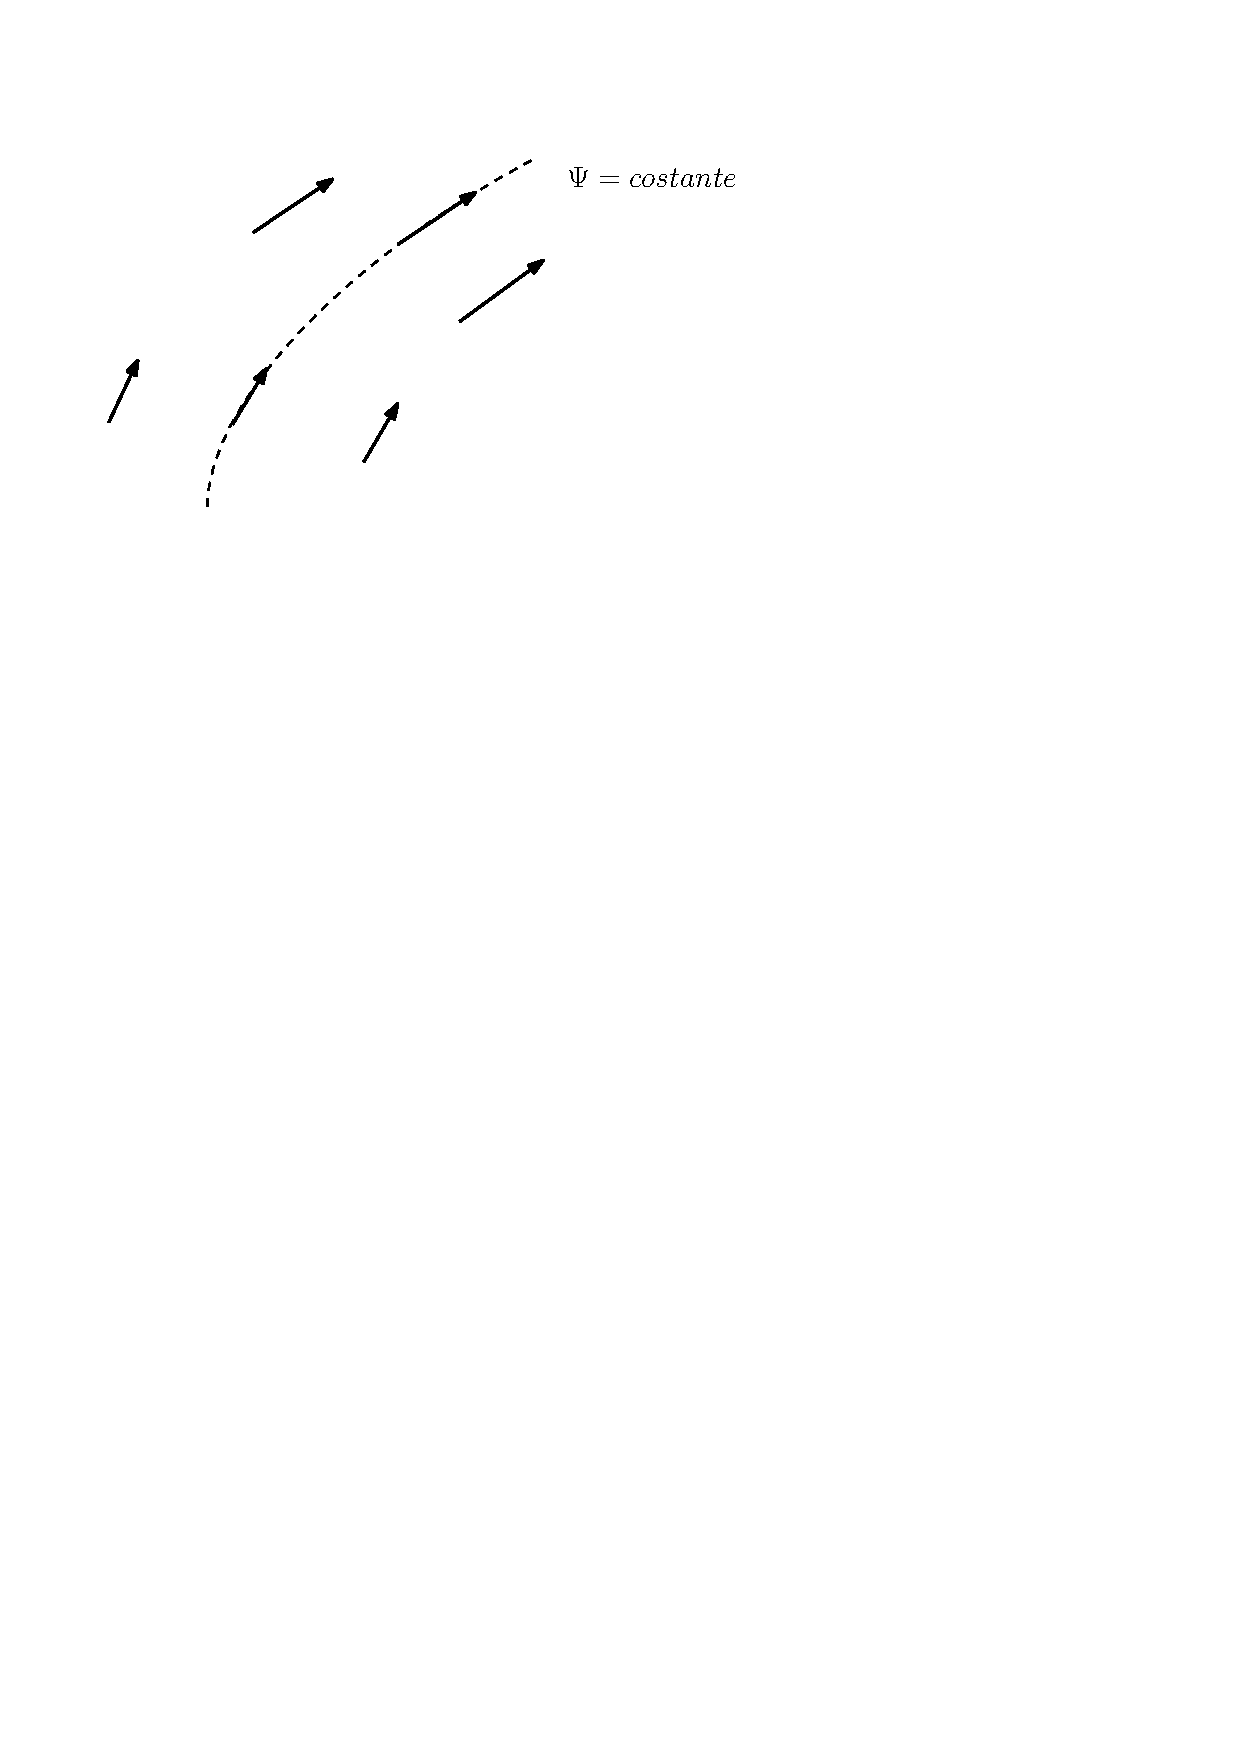
\includegraphics[scale=0.9]{./3.5 Equazioni di Navier-Stokes/3.5-1}
		\centering
		\caption{Linea di corrente e vettori velocità}
	\end{figure}
%

\begin{equation*}
	\begin{gathered}
		\Psi = costante \rightarrow \Psi_x \dd{x} + \Psi_y \dd{y} = 0\\
		\text{Sostituendo}\\
		- v \dd{x} + u \dd{y} = 0\\
		\text{quindi}\\
		\frac{v}{u} = \frac{\dd{y}}{\dd{x}} \rightarrow \begin{bmatrix} u & v \end{bmatrix} \propto  \begin{bmatrix} \dd{x} & \dd{y} \end{bmatrix}
	\end{gathered}
\end{equation*}

Quindi se la funzione di flusso è costante, la tangente alla linea di corrente è parallela al vettore di velocità, dai quali si ottiene la linea di corrente.
Si può anche effettuare il procedimento ``al contrario''.

\subsection*{Bibliografia 3.6}
\cite[Cap.\ 9.1, 9.2, 9.3, 9.4, 9.5]{CengelCimbala}\\
\cite[Cap.\ 5.6, 5.8, 5.9, 5.11]{PnueliGutfinger}